\documentclass[12pt]{report}
\usepackage[utf8]{inputenc}
\usepackage[margin=1.2in]{geometry}
\usepackage{graphicx}
\usepackage{float}
\usepackage{subcaption}
\usepackage{amsmath}
\usepackage{amssymb}
\usepackage{ulem}
\usepackage{bm}
\usepackage{framed}
\usepackage{xcolor}
\usepackage{ragged2e}
\usepackage{color}
\usepackage{soul}
\usepackage{cancel}
\graphicspath{ {images/} }
\setlength{\parskip}{1em}
\allowdisplaybreaks


\usepackage{titling}
\newcommand{\subtitle}[1]{%
	\posttitle{%
		\par\end{center}
	\begin{center}\large#1\end{center}
	\vskip0.5em}%
}

\newenvironment{blueframed}[1][blue]
{\def\FrameCommand{\fboxsep=\FrameSep\fcolorbox{#1}{white}}%
\MakeFramed {\advance\hsize-\width \FrameRestore}}
{\endMakeFramed}

\newenvironment{spmatrix}[1]
{\def\mysubscript{#1}\mathop\bgroup\begin{bmatrix}}
{\end{bmatrix}\egroup_{\textstyle\mathstrut\mysubscript}}

\title{Tutorial 11}
\subtitle
{
\textbf{keywords}: time series,AR model, GDP, growth rate, residual plot, correlogram, white noise, Breusch-Godfrey test for serial correlation, F-test

\textbf{estimated reading time}: 38 minutes
}
\author{Quang Bui}
\date{October 9, 2018}

\begin{document}

\maketitle

\section*{Question 1}
\noindent (Complete in class)


\newpage
\section*{Question 2}
\noindent \textit{A dynamically well-specified model is the one with no evidence of serial correlation in its errors.}

\noindent EViews workfile: \textit{US\_gdp.wf1}

\noindent \textit{US\_gdp.wf1} contains quarterly data during the period 1954Q1 and 2017Q2:
\begin{align*}
gdp &- U.S.\ real\ Gross\ Domestic\ Product\ (\$\ billions)
\end{align*}

\noindent \textcolor{red}
{
	(a) Create the quarterly GDP annualised growth rate using logarithmic transformation and differencing. Denote the series $dlgdp$.
}

%\noindent \textit{To obtain annualised quarterly real U.S. GDP growth in EViews, click on `Genr' on the workfile toolbar and in the dialogue box that appears type} $dlgdp=(log(gdp)-log(gdp(-1)))^*400$.

\noindent The \textbf{first difference of} $\boldsymbol{log(gdp_t)}$, $$\Delta log(gdp_t) = log(gdp_t)-log(gdp_{t-1})$$ is the approximate proportional change in quarterly real GDP,
\begin{align*}
	\Delta log(gdp_t) &= log(gdp_t)-log(gdp_{t-1}) \\
	&\approx \dfrac{gdp_t - gdp_{t-1}}{gdp_{t-1}}
\end{align*} Multiplying 100 to $\Delta log(gdp_t)$ gives the percentage change in quarterly real GDP i.e. quarterly real GDP growth rate, \begin{align*}
100\Delta log(gdp_t) &\approx 100\times \dfrac{gdp_t - gdp_{t-1}}{gdp_{t-1}} \\
&=\%\Delta gdp_t
\end{align*} 
\noindent To annualise the quarterly real GDP growth rate, we multiply the quarterly real GDP growth rate by 4, \begin{align*}
	dlgdp_t&=4\times 100\Delta log(gdp_t) \\
	&=400\Delta log(gdp_t)
\end{align*} Note based on Farshid's response on Discussion Forum (2017 Sem2 I think): \\ $100^*\big(log(gdp_t) - log(gdp_{t-4})\big)$ is percentage change in real GDP relative to the same quarter of last year i.e. annual GDP growth. For econometric analysis, we use $400^*\big(log(gdp_t) - log(gdp_{t-1}\big)$ which is one quarter growth rate multiplied by 4 to annualise it when there is no seasonality in that data and $100^*\big(log(gdp_t) - log(gdp_{t-4})\big)$ only when the data is seasonal. Since $log(gdp_t)$ is not seasonal, we use the annualise quarterly real GDP growth. (Outside scope of unit.)

\noindent To generate the annualised quarterly real GDP growth rate from the Command window in EViews, $$genr\ dlgdp=(log(gdp)-log(gdp(-1)))^*400$$
\begin{figure}[H]
	\centerline{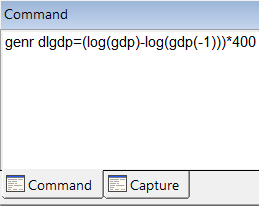
\includegraphics{tute11_2}}
\end{figure}
\vspace{-\baselineskip}
\begin{figure}[H]
	\centerline{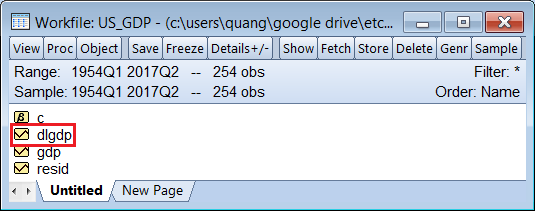
\includegraphics{tute11_3}}
\end{figure}
\vspace{-\baselineskip}


%%%%%%%%%% TABLE OBJECT %%%%%%%%%%
\begin{table}[H]
	\centering
	\begin{tabular}{lr}
		\multicolumn{1}{c}{}&\multicolumn{1}{r}{$dlgdp$}\\
		\multicolumn{1}{c}{1954Q1}&\multicolumn{1}{r}{$NA$}\\
		\multicolumn{1}{c}{1954Q2}&\multicolumn{1}{r}{$0.426987$}\\
		\multicolumn{1}{c}{1954Q3}&\multicolumn{1}{r}{$4.510765$}\\
		\multicolumn{1}{c}{1954Q4}&\multicolumn{1}{r}{$7.723652$}\\
		\multicolumn{1}{c}{\vdots}&\multicolumn{1}{r}{\vdots}\\
		\multicolumn{1}{c}{2016Q4}&\multicolumn{1}{r}{$1.743710$}\\
		\multicolumn{1}{c}{2017Q1}&\multicolumn{1}{r}{$1.227685$}\\
		\multicolumn{1}{c}{2017Q2}&\multicolumn{1}{r}{$2.535842$}\\
	\end{tabular}
	\caption{Annualised quarterly U.S. GDP growth for the period 1954Q2 to 2017Q2. The first observation is lost because of first differencing.}
	%\label{tab:}
\end{table}

\newpage
\noindent \textcolor{red}
{
	(b) Truncate the sample such that you consider data ranging from $1955Q1$ to $2017Q2$. Estimate the following OLS regression (which is annualised quarterly U.S. GDP growth modelled with an AR(2) process): $$dlgdp_t = \varphi_0 + \varphi_1dlgdp_{t-1} + \varphi_2dlgdp_{t-2} + u_t$$
}
\noindent To change the sample from the Command window, $$smpl\ 1955Q1\ 2017Q2$$
\begin{figure}[H]
	\centerline{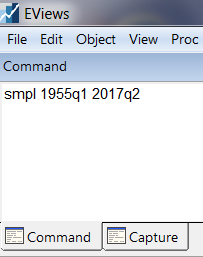
\includegraphics{q3_2}}
\end{figure}
\vspace{-\baselineskip}
\begin{figure}[H]
	\centerline{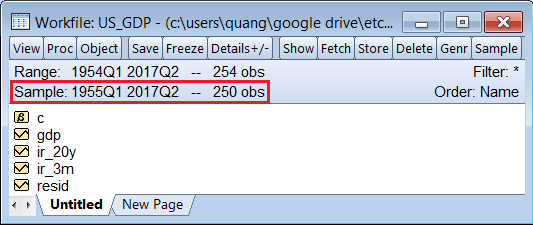
\includegraphics{q3_3}}
\end{figure}
\vspace{-\baselineskip}
\noindent Notice that the sample (but not the range) has changed in the status window. \textit{Do not change the workfile range in the status window.}

\newpage
\noindent To estimate $dlgdp_t = \varphi_0 + \varphi_1dlgdp_{t-1} + \varphi_2dlgdp_{t-2} + u_t$ and name the equation $ar2$ from the Command window in EViews, 
$$equation\ ar2.ls\ dlgdp\ c\ dlgdp(\text{-}1to\text{-2})$$
\begin{figure}[H]
	\centerline{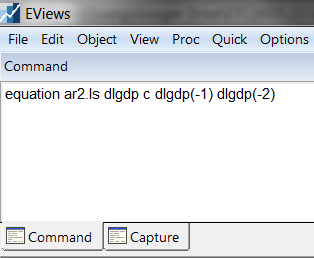
\includegraphics{tute11_1}}
\end{figure}
\vspace{-\baselineskip}

%%%%%%%%%% TABLE OBJECT %%%%%%%%%%
\begin{table}[H]
	\centering
	\begin{tabular}{lrrrr}
		\multicolumn{3}{l}{Dependent Variable: DLGDP}&\multicolumn{1}{c}{}&\multicolumn{1}{c}{}\\
		\multicolumn{3}{l}{Method: Least Squares}&\multicolumn{1}{c}{}&\multicolumn{1}{c}{}\\
		\multicolumn{3}{l}{Sample: 1955Q1 2017Q2}&\multicolumn{1}{c}{}&\multicolumn{1}{c}{}\\
		\multicolumn{3}{l}{Included observations: 250}&\multicolumn{1}{c}{}&\multicolumn{1}{c}{}\\
		[4.5pt] \hline \\ [-4.5pt]
		\multicolumn{1}{c}{Variable}&\multicolumn{1}{r}{Coefficient}&\multicolumn{1}{r}{Std. Error}&\multicolumn{1}{r}{t-Statistic}&\multicolumn{1}{r}{Prob.}\\
		[4.5pt] \hline \\ [-4.5pt]
		\multicolumn{1}{c}{C}&\multicolumn{1}{r}{$1.742741$}&\multicolumn{1}{r}{$0.300922$}&\multicolumn{1}{r}{$5.791343$}&\multicolumn{1}{r}{$0.0000$}\\
		\multicolumn{1}{c}{DLGDP(-1)}&\multicolumn{1}{r}{$0.306892$}&\multicolumn{1}{r}{$0.063042$}&\multicolumn{1}{r}{$4.868049$}&\multicolumn{1}{r}{$0.0000$}\\
		\multicolumn{1}{c}{DLGDP(-2)}&\multicolumn{1}{r}{$0.108769$}&\multicolumn{1}{r}{$0.063053$}&\multicolumn{1}{r}{$1.725045$}&\multicolumn{1}{r}{$0.0858$}\\
		[4.5pt] \hline \\ [-4.5pt]
		\multicolumn{1}{l}{R-squared}&\multicolumn{1}{r}{$0.130079$}&\multicolumn{2}{l}{Mean dependent var}&\multicolumn{1}{r}{$2.999617$}\\
		\multicolumn{1}{l}{Adjusted R-squared}&\multicolumn{1}{r}{$0.123035$}&\multicolumn{2}{l}{S.D. dependent var}&\multicolumn{1}{r}{$3.499670$}\\
		\multicolumn{1}{l}{S.E. of regression}&\multicolumn{1}{r}{$3.277315$}&\multicolumn{2}{l}{Akaike info criterion}&\multicolumn{1}{r}{$5.223854$}\\
		\multicolumn{1}{l}{Sum squared resid}&\multicolumn{1}{r}{$2652.976$}&\multicolumn{2}{l}{Schwarz criterion}&\multicolumn{1}{r}{$5.266111$}\\
		\multicolumn{1}{l}{Log likelihood}&\multicolumn{1}{r}{$-649.9817$}&\multicolumn{2}{l}{Hannan-Quinn criter.}&\multicolumn{1}{r}{$5.240861$}\\
		\multicolumn{1}{l}{F-statistic}&\multicolumn{1}{r}{$18.46692$}&\multicolumn{2}{l}{Durbin-Watson stat}&\multicolumn{1}{r}{$1.999001$}\\
		\multicolumn{1}{l}{Prob(F-statistic)}&\multicolumn{1}{r}{$0.000000$}&\multicolumn{1}{c}{}&\multicolumn{1}{c}{}&\multicolumn{1}{c}{}\\
		[4.5pt] \hline \\ [-4.5pt]
	\end{tabular}
	%\caption{Add your caption here.}
	%\label{tab:}
	$$\widehat{dlgdp}_t = \underset{(0.3009)}{1.7427} + \underset{(0.0630)}{0.3069}dlgdp_{t-1} + \underset{(0.0631)}{0.1088}dlgdp_{t-2}$$
\end{table}



\newpage
\justify \noindent \textcolor{red}{(c) Inspect the time plot and the correlogram of the residuals associated with the estimated model. Is there any visual evidence that the dynamics of the model is not specified well?}

\noindent We want to check if there is evidence of serially correlated errors, $$cov(u_t, u_{t-j}) \neq 0 \quad for\ j=1,2,\dots$$ by inspecting the line graph of the OLS residuals. 

\noindent To obtain a line graph of the residuals from the estimated AR(2) model of annualised quarterly real U.S. GDP growth in EViews, $$\widehat{dlgdp}_t = \underset{(0.3009)}{1.7427} + \underset{(0.0630)}{0.3069}dlgdp_{t-1} + \underset{(0.0631)}{0.1088}dlgdp_{t-2}$$
$$AR2 \to View\ to\ Actual,Fitted,Residual \to Residual\ Graph$$
\begin{figure}[H]
	\centerline{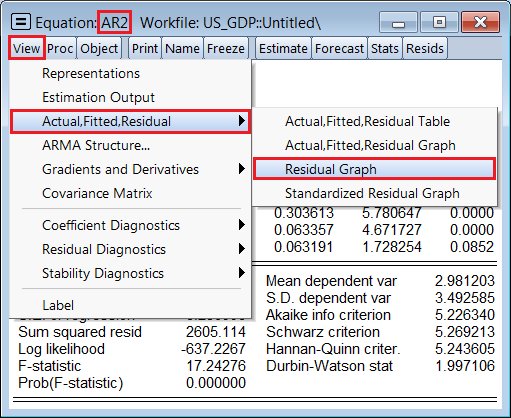
\includegraphics{tute11_5}}
\end{figure}
\vspace{-\baselineskip}
\begin{figure}[H]
	\centerline{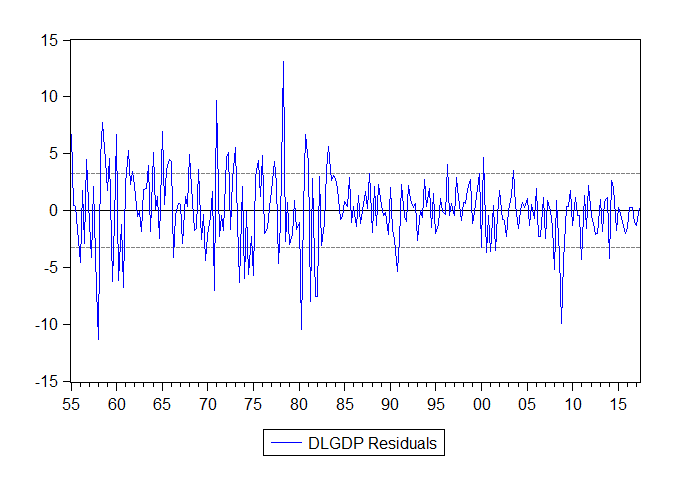
\includegraphics{tute11_6}}
\end{figure}
\vspace{-\baselineskip}
\noindent We can detect a slight pattern in the evolution of residuals but it does not necessarily persist over time. It is not clear if the errors are serially correlated from visual inspection. The correlogram gives us better information, $$AR2 \to View \to Residual\ Diagnostics \to Correlogram\ Q-statistics$$
\begin{figure}[H]
	\centerline{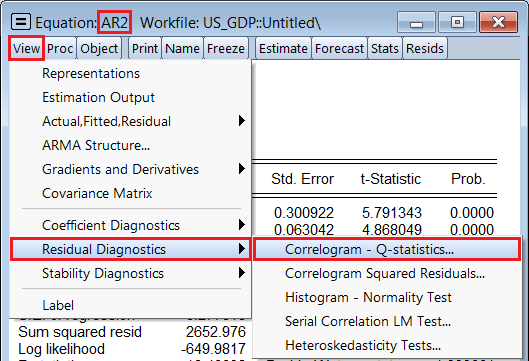
\includegraphics{tute11_25}}
\end{figure}
\vspace{-\baselineskip}
\begin{figure}[H]
	\centerline{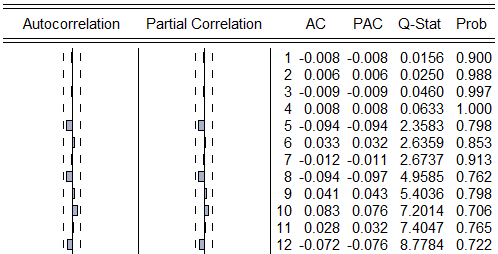
\includegraphics{tute11_26}}
\end{figure}
\vspace{-\baselineskip}
\noindent and shows no evidence of serial correlation in the errors.


\noindent \textcolor{red}{(d) Test for autocorrelation (serially correlation) in the errors of the model, $$dlgdp_t = \varphi_0 + \varphi_1dlgdp_{t-1} + \varphi_2dlgdp_{t-2} + u_t$$ by using the Breusch-Godfrey test (include 8 lags for this test). Discuss your results.}

\noindent Since our time series data is quarterly, testing up to 8 lags covers two years.

\noindent We are testing for serial correlation in $u_t$ of order 8, so we specify a model of $dlgdp$ with errors that follow an AR(8) process.
\begin{align*}
dlgdp_t &= \varphi_0 + \varphi_1dlgdp_{t-1} + \varphi_2dlgdp_{t-2} + u_t \\
u_t &= \rho_1u_{t-1} + \rho_2u_{t-2} + \rho_3u_{t-3} + \dots + \rho_7u_{t-7} + \rho_8u_{t-8} + e_t
\end{align*} $$\{e_t, t=1,2,\dots,n \sim i.i.d(0,\sigma^2)\}$$ where $e_t$ for $t=1,2,\dots,n$ are independent and identically distributed with mean 0 and variance $\sigma^2$
\begin{align*}
H_0&: \rho_1 = \rho_2 = \rho_3 = \dots = \rho_8 = 0 \\
H_1&: at\ least\ one\ of\ the\ above\ \rho \neq 0
\end{align*}
To perform the Breusch-Godfrey test for serial correlation in the errors of model of $dlgdp$ at any lag up to and include lag 8 (8th order serial correlation),
\begin{itemize}
	\item Estimate the model $$dlgdp_t = \varphi_0 + \varphi_1dlgdp_{t-1} + \varphi_2dlgdp_{t-2} + u_t$$
	\item Save the residuals from the above estimated model 
	\item Then estimate the following $auxiliary\ regression \dots$ $$\hat{u}_t = \alpha_0 + \alpha_1dlgdp_{t-1} + \alpha_2dlgdp_{t-2} + \rho_1\hat{u}_{t-1} + \rho_2\hat{u}_{t-2} + \dots + \rho_8\hat{u}_{t-8} + v_t$$
	\item We're testing the null hypothesis that there is no serial correlation in the errors at any lag up to and include lag 8, against the alternative hypothesis that there is serial correlation in the errors in at least one lag up to and including lag 8.
	\item Compare the calculated test statistics with the critical value and conclude if there is evidence of serial correlation in the errors in at least one lag up to and including lag 8.
\end{itemize}

\noindent Generate the residuals from the estimated model of $dlgdp$, $$AR2 \to Proc \to Make\ Residual\ Series$$
\begin{figure}[H]
	\centerline{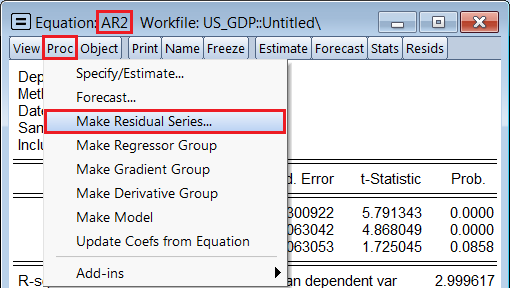
\includegraphics{tute11_27}}
\end{figure}
\vspace{-\baselineskip} \noindent and name the residual series $uhat$,
\begin{figure}[H]
	\centerline{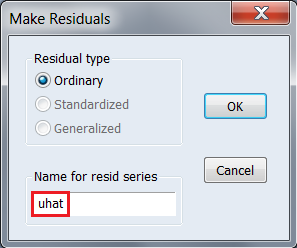
\includegraphics{tute11_28}}
\end{figure}
\vspace{-\baselineskip} \noindent then estimated the following auxiliary regression, $$\hat{u}_t = \alpha_0 + \alpha_1dlgdp_{t-1} + \alpha_2dlgdp_{t-2} + \rho_1\hat{u}_{t-1} + \rho_2\hat{u}_{t-2} + \dots + \rho_7\hat{u}_{t-7} + \rho_8\hat{u}_{t-8} + v_t$$ $$ls\ uhat\ c\ dlgdp(-1)\ dlgdp(-2)\ uhat(-1to-8)$$ \begin{figure}[H]
	\centerline{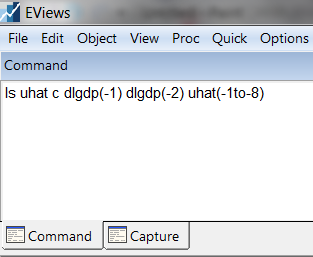
\includegraphics{tute11_29}}
\end{figure}
\vspace{-\baselineskip}
%%%%%%%%%% TABLE OBJECT %%%%%%%%%%
\begin{table}[H]
	\centering
	\begin{tabular}{lrrrr}
		\multicolumn{3}{l}{Dependent Variable: UHAT}&\multicolumn{1}{c}{}&\multicolumn{1}{c}{}\\
		%\multicolumn{3}{l}{Method: Least Squares}&\multicolumn{1}{c}{}&\multicolumn{1}{c}{}\\
		\multicolumn{4}{l}{Sample (adjusted): 1957Q1 2017Q2}&\multicolumn{1}{c}{}\\
		\multicolumn{5}{l}{Included observations: 242 after adjustments}\\
		[4.5pt] \hline \\ [-4.5pt]
		\multicolumn{1}{c}{Variable}&\multicolumn{1}{r}{Coefficient}&\multicolumn{1}{r}{Std. Error}&\multicolumn{1}{r}{t-Statistic}&\multicolumn{1}{r}{Prob.}\\
		[4.5pt] \hline \\ [-4.5pt]
		\multicolumn{1}{c}{C}&\multicolumn{1}{r}{$12162.92$}&\multicolumn{1}{r}{$36065.18$}&\multicolumn{1}{r}{$0.337248$}&\multicolumn{1}{r}{$0.7362$}\\
		\multicolumn{1}{c}{DLGDP(-1)}&\multicolumn{1}{r}{$-8468.594$}&\multicolumn{1}{r}{$25065.25$}&\multicolumn{1}{r}{$-0.337862$}&\multicolumn{1}{r}{$0.7358$}\\
		\multicolumn{1}{c}{DLGDP(-2)}&\multicolumn{1}{r}{$4390.371$}&\multicolumn{1}{r}{$12972.63$}&\multicolumn{1}{r}{$0.338433$}&\multicolumn{1}{r}{$0.7353$}\\
		\multicolumn{1}{c}{UHAT(-1)}&\multicolumn{1}{r}{$8468.599$}&\multicolumn{1}{r}{$25065.24$}&\multicolumn{1}{r}{$0.337862$}&\multicolumn{1}{r}{$0.7358$}\\
		\multicolumn{1}{c}{UHAT(-2)}&\multicolumn{1}{r}{$-1791.427$}&\multicolumn{1}{r}{$5280.311$}&\multicolumn{1}{r}{$-0.339265$}&\multicolumn{1}{r}{$0.7347$}\\
		\multicolumn{1}{c}{UHAT(-3)}&\multicolumn{1}{r}{$371.3373$}&\multicolumn{1}{r}{$1105.837$}&\multicolumn{1}{r}{$0.335797$}&\multicolumn{1}{r}{$0.7373$}\\
		\multicolumn{1}{c}{UHAT(-4)}&\multicolumn{1}{r}{$-80.86302$}&\multicolumn{1}{r}{$234.9714$}&\multicolumn{1}{r}{$-0.344140$}&\multicolumn{1}{r}{$0.7311$}\\
		\multicolumn{1}{c}{UHAT(-5)}&\multicolumn{1}{r}{$15.46959$}&\multicolumn{1}{r}{$48.18367$}&\multicolumn{1}{r}{$0.321055$}&\multicolumn{1}{r}{$0.7485$}\\
		\multicolumn{1}{c}{UHAT(-6)}&\multicolumn{1}{r}{$-3.979231$}&\multicolumn{1}{r}{$10.78031$}&\multicolumn{1}{r}{$-0.369120$}&\multicolumn{1}{r}{$0.7124$}\\
		\multicolumn{1}{c}{UHAT(-7)}&\multicolumn{1}{r}{$0.436618$}&\multicolumn{1}{r}{$1.947329$}&\multicolumn{1}{r}{$0.224214$}&\multicolumn{1}{r}{$0.8228$}\\
		\multicolumn{1}{c}{UHAT(-8)}&\multicolumn{1}{r}{$-0.392500$}&\multicolumn{1}{r}{$0.591407$}&\multicolumn{1}{r}{$-0.663671$}&\multicolumn{1}{r}{$0.5076$}\\
		[4.5pt] \hline \\ [-4.5pt]
		\multicolumn{1}{l}{R-squared}&\multicolumn{1}{r}{$0.026798$}&\multicolumn{2}{l}{Mean dependent var}&\multicolumn{1}{r}{$-0.018619$}\\
		\multicolumn{1}{l}{Adjusted R-squared}&\multicolumn{1}{r}{$-0.015331$}&\multicolumn{2}{l}{S.D. dependent var}&\multicolumn{1}{r}{$3.254370$}\\
		\multicolumn{1}{l}{S.E. of regression}&\multicolumn{1}{r}{$3.279223$}&\multicolumn{2}{l}{Akaike info criterion}&\multicolumn{1}{r}{$5.257479$}\\
		\multicolumn{1}{l}{Sum squared resid}&\multicolumn{1}{r}{$2484.012$}&\multicolumn{2}{l}{Schwarz criterion}&\multicolumn{1}{r}{$5.416067$}\\
		\multicolumn{1}{l}{Log likelihood}&\multicolumn{1}{r}{$-625.1549$}&\multicolumn{2}{l}{Hannan-Quinn criter.}&\multicolumn{1}{r}{$5.321364$}\\
		\multicolumn{1}{l}{F-statistic}&\multicolumn{1}{r}{$0.636091$}&\multicolumn{2}{l}{Durbin-Watson stat}&\multicolumn{1}{r}{$1.994378$}\\
		\multicolumn{1}{l}{Prob(F-statistic)}&\multicolumn{1}{r}{$0.782138$}&\multicolumn{1}{c}{}&\multicolumn{1}{c}{}&\multicolumn{1}{c}{}\\
		[4.5pt] \hline \\ [-4.5pt]
	\end{tabular}
	%\caption{Add your caption here.}
	%\label{tab:}
\end{table}

$$(Type\ out\ estimated\ aux)$$
\noindent The BG test statistic under the null,
$$BG = (n-8)\times R^2_{\hat{u}} \overset{asy}{\sim} \chi^2_8 \quad under\ H_0$$
\noindent The calculated BG test statistic,
$$BG_{calc} = (250-8) \times 0.02680 = 6.4851$$
\noindent The critical value, $$scalar\ cv=@qchisq(0.95,8)$$ \begin{figure}[H]
	\centerline{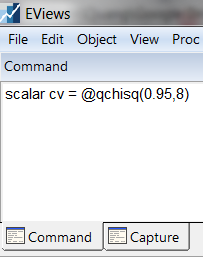
\includegraphics{tute11_30}}
\end{figure}
\vspace{-\baselineskip} \begin{figure}[H]
	\centerline{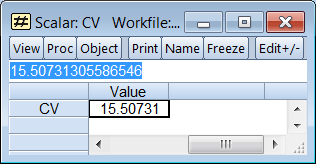
\includegraphics{tute11_31}}
\end{figure}
\vspace{-\baselineskip}
$$BG_{crit} = \chi^2_{0.95,8} = 15.5073$$

\noindent Since $BG_{calc} = 6.4851 < BG_{crit} = 15.5073$ we fail to reject the null and conclude that there is insufficient evidence from the sample to suggest that there is serial correlation in the errors in at least one lag up to and include the 8th lag.

\noindent Note: The EViews inbuilt BG test produces different values as it sets the missing values of the lagged residuals to 0 so that there are no missing observations and $q$ becomes 0. The official tutorial solution has used the inbuilt BG test which gives $BG_{calc} = 8.972$.




\newpage
\section*{Question 3}
\noindent \textit{We can use usual econometric tools in a dynamically well-specified model.}

\noindent Early warning systems are very useful for policy makers. In economics, variables which can give us advanced warning that the economy may be slowing down in 3 months to a year ahead are very useful. Such variables are called ``leading indicators". The ``interest rate spread", $$spread = ir\_20y - ir\_3m$$ which is the difference between the long term and short interest rates, is believed to be a leading indicator.  When the spread becomes very small or even negative, it means that confidence in the long-term prospects of the economy is low, which warns of a possible low growth period or even a recession ahead. 

\noindent The data file used in the previous section \textit{US\_gdp.wf1} contains quarterly observations on: 
\begin{align*}
gdp &- U.S.\ real\ Gross\ Domestic\ Product\ (\$\ billions)\\
ir\_3m &- U.S.\ 3\text{-}month\ Treasury\ bill\ interest\ rates\ (\%) \\
ir\_20y &- U.S.\ 20\text{-}year\ Government\ bond\ yields\ (\%)
\end{align*}
\noindent You have already created $dlgdp$.

\noindent \textcolor{red}{a) Switch the sample back to 1954Q1 and 2017Q2 and generate a new variable called $spread = ir\_20y - ir\_3m$. Is $spread$ white noise? Is it mean-reverting? Does its correlogram suggest that $spread$ is stationary?}

\noindent To change the sample from the Command window, $$smpl\ 1954Q1\ 2017Q2$$
\begin{figure}[H]
	\centerline{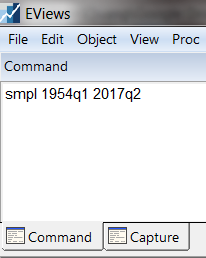
\includegraphics{tute11_32}}
\end{figure}
\vspace{-\baselineskip}
\begin{figure}[H]
	\centerline{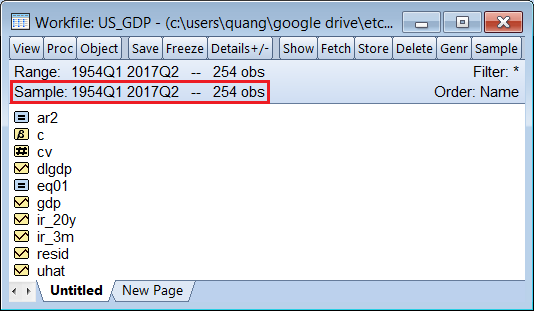
\includegraphics{tute11_33}}
\end{figure}
\vspace{-\baselineskip}
\noindent Notice that the sample (but not the range) has changed in the status window. \textit{Do not change the workfile range in the status window.}

\noindent To generate the $spread$ variable from the Command window, $$genr\ spread=ir\_20y-ir\_3m$$
\begin{figure}[H]
	\centerline{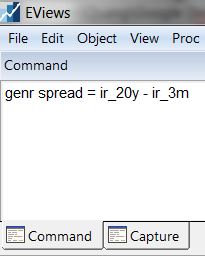
\includegraphics{tute11_34}}
\end{figure}
\vspace{-\baselineskip}
\begin{figure}[H]
	\centerline{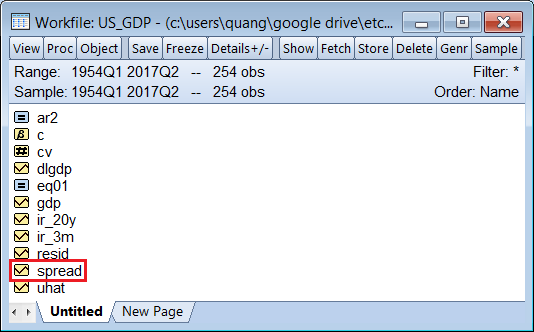
\includegraphics{tute11_35}}
\end{figure}
\vspace{-\baselineskip}

\noindent \uline{Is $spread$ white noise? Is it mean-reverting?}

\noindent Inspecting the line graph of $spread$ can help us determine whether it is white noise and if it is mean-reverting. To obtain a line graph of $spread$ from the Command window, $$plot\ spread$$
\begin{figure}[H]
	\centerline{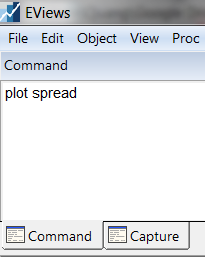
\includegraphics{tute11_36}}
\end{figure}
\vspace{-\baselineskip}
\begin{figure}[H]
	\centerline{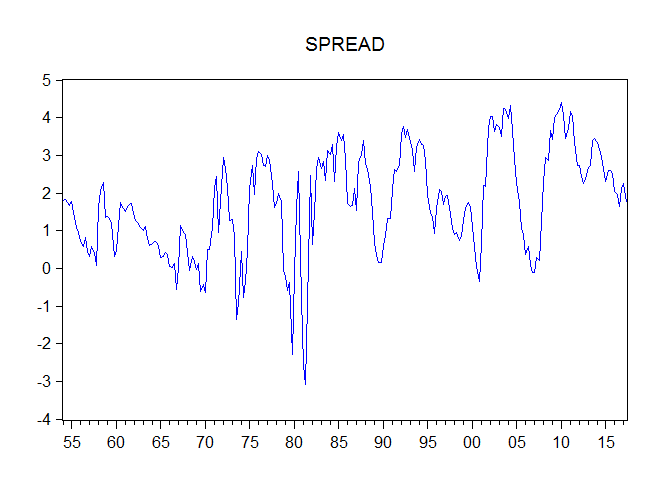
\includegraphics{tute11_37}}
\end{figure}
\vspace{-\baselineskip} \noindent We can see long swings in the term spread which would suggest that it is not white noise. Although the term spread tends to revert back to its mean, it has some persistence (autocorrelation).


\noindent From the correlogram of $spread$ $$spread \to Correlogram$$ \begin{figure}[H]
	\centerline{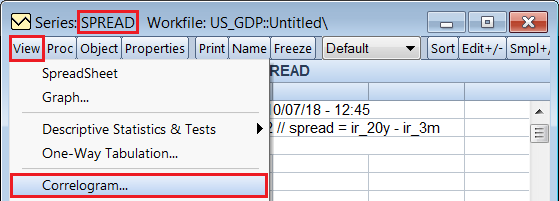
\includegraphics{tute11_38}}
\end{figure}
\vspace{-\baselineskip} \begin{figure}[H]
	\centerline{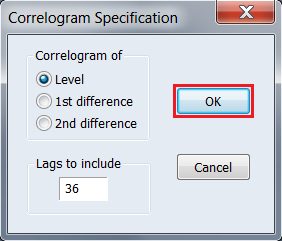
\includegraphics{tute11_39}}
\end{figure}
\vspace{-\baselineskip} \begin{figure}[H]
	\centerline{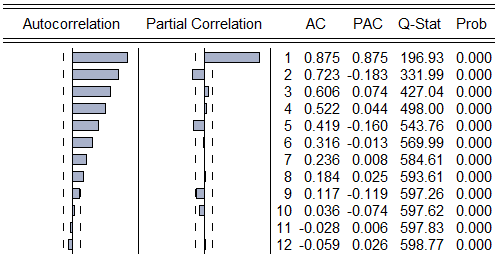
\includegraphics{tute11_40}}
\end{figure}
\vspace{-\baselineskip} \noindent we find that the sample autocorrelation coefficients of $spread$ is statistically significantly different from 0 (up to and including the 8th lag, the sample autocorrelation coefficients lie outside the 2 standard error bands) which indicates that it is not white noise.

\noindent \uline{Does the correlogram suggest that $spread$ is stationary?}

\justify
\begin{blueframed}
	\textcolor{blue}{\textbf{Background}}
	\vspace{-\baselineskip}
	\justify
	\textcolor{blue}{\underline{Stationary time series process}}
	
	\noindent \textcolor{blue}
	{
		A stationary time series process has the following properties,
		\begin{align*}
		E(y_t) &= \mu \quad for\ all\ t\ \Rightarrow the\ mean\ is\ time\ invariant \\
		Var(y_t) &= \gamma_0 \quad for\ all\ t\ \Rightarrow the\ variance\ is\ time\ invariant \\
		Cov(y_t,y_{t-j}) &= \gamma_j \quad for\ all\ t\ and\ j \\
		&\Downarrow \\
		&the\ covariance\ of\ y_t\ and\ y_{t-j}\ only\ depends\ on\ the \\
		&time\ interval\ separating\ them\ i.e.\ only\ j\ and\ not\ t 
		\end{align*}
	}
\end{blueframed}
\justify
\begin{blueframed}
	
	\noindent \textcolor{blue}
	{
		If any of these stationary properties/assumptions are violated then we have a non-stationary time series. \\ \\
		%\uline{Unit Root process} \\ \\
		\uline{Random Walk process} \\ \\
		A random walk process is an AR(1) process with a unit root i.e. a special case of a unit root process. If the long-term interest rate $ir\_20y$ is a random walk process then it will assume the following model, $$ir\_20y_t = ir\_20y_{t-1} + u_t$$ $$where\ u_t \sim i.i.d(0,\sigma^2)$$
		As we can see, it has the same form as an AR(1) model (without a constant) where $\varphi_1=1$ 
		$$ir\_20y_t = c + \varphi_1ir\_20y_{t-1} + u_t$$
		$$\downarrow$$ $$ir\_20y_t = \cancel{c} + 1\times ir\_20y_{t-1} + u_t$$
		$$\downarrow$$
		$$ir\_20y_t = ir\_20y_{t-1} + u_t$$ If a time series process is a random walk process then it is non-stationary.
	}
\end{blueframed}



\noindent From the correlogram of $spread$, we find that the sample autocorrelation coefficient declines exponentially which indicates that $spread$ is stationary.  If $spread$ declines very slowly, then $spread$ is said to be a unit root process (a unit root process is non-stationary and has high persistence).

\noindent \textcolor{red}{b) In order to investigate the leading indicator property of $spread$, use data from \textit{1955q1 to 2017q2} to estimate the following model (ARDL(2,2)): $$dlgdp_t = \beta_0 + \beta_1dlgdp_{t-1} + \beta_2dlgdp_{t-2} + \beta_3spread_{t-1} + \beta_4spread_{t-2} + u_t$$ and test the joint significance of $spread_{t-1}$ and $spread_{t-2}$ at the 5\% level of significance. What are the null and alternative hypothesis? What is the restricted model? What is the test statistics and its distribution under the null? Perform the test and state your conclusion.}

\noindent To change the sample from the Command window, $$smpl\ 1955Q1\ 2017Q2$$
\begin{figure}[H]
	\centerline{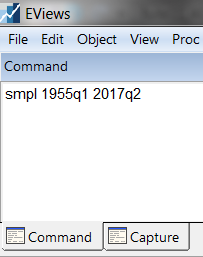
\includegraphics{tute11_41}}
\end{figure}
\vspace{-\baselineskip}
\begin{figure}[H]
	\centerline{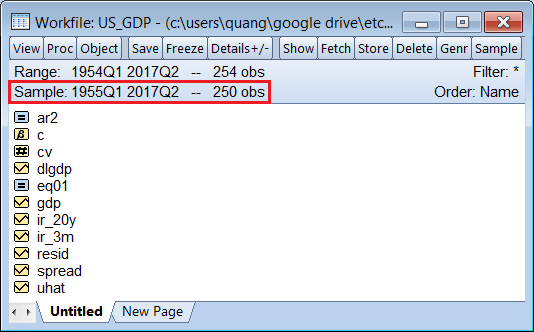
\includegraphics{tute11_43}}
\end{figure}
\vspace{-\baselineskip} \noindent To estimate the ARDL(2,2) model of $dlgdp$ from the Command window, $$ls\ c\ dlgdp(-1to-2)\ spread(-1to-2)$$
\begin{figure}[H]
	\centerline{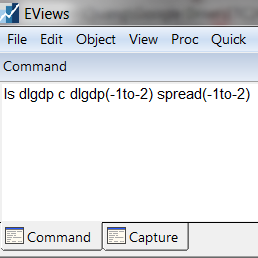
\includegraphics{tute11_42}}
\end{figure}
\vspace{-\baselineskip}
%%%%%%%%%% TABLE OBJECT %%%%%%%%%%
\begin{table}[H]
	\centering
	\begin{tabular}{lrrrr}
		\multicolumn{3}{l}{Dependent Variable: DLGDP}&\multicolumn{1}{c}{}&\multicolumn{1}{c}{}\\
		\multicolumn{3}{l}{Method: Least Squares}&\multicolumn{1}{c}{}&\multicolumn{1}{c}{}\\
		\multicolumn{3}{l}{Sample: 1955Q1 2017Q2}&\multicolumn{1}{c}{}&\multicolumn{1}{c}{}\\
		\multicolumn{3}{l}{Included observations: 250}&\multicolumn{1}{c}{}&\multicolumn{1}{c}{}\\
		[4.5pt] \hline \\ [-4.5pt]
		\multicolumn{1}{c}{Variable}&\multicolumn{1}{r}{Coefficient}&\multicolumn{1}{r}{Std. Error}&\multicolumn{1}{r}{t-Statistic}&\multicolumn{1}{r}{Prob.}\\
		[4.5pt] \hline \\ [-4.5pt]
		\multicolumn{1}{c}{C}&\multicolumn{1}{r}{$1.103416$}&\multicolumn{1}{r}{$0.394741$}&\multicolumn{1}{r}{$2.795293$}&\multicolumn{1}{r}{$0.0056$}\\
		\multicolumn{1}{c}{DLGDP(-1)}&\multicolumn{1}{r}{$0.277960$}&\multicolumn{1}{r}{$0.063335$}&\multicolumn{1}{r}{$4.388718$}&\multicolumn{1}{r}{$0.0000$}\\
		\multicolumn{1}{c}{DLGDP(-2)}&\multicolumn{1}{r}{$0.107821$}&\multicolumn{1}{r}{$0.062999$}&\multicolumn{1}{r}{$1.711453$}&\multicolumn{1}{r}{$0.0883$}\\
		\multicolumn{1}{c}{SPREAD(-1)}&\multicolumn{1}{r}{$-0.122029$}&\multicolumn{1}{r}{$0.315459$}&\multicolumn{1}{r}{$-0.386831$}&\multicolumn{1}{r}{$0.6992$}\\
		\multicolumn{1}{c}{SPREAD(-2)}&\multicolumn{1}{r}{$0.547081$}&\multicolumn{1}{r}{$0.317431$}&\multicolumn{1}{r}{$1.723466$}&\multicolumn{1}{r}{$0.0861$}\\
		[4.5pt] \hline \\ [-4.5pt]
		\multicolumn{1}{l}{R-squared}&\multicolumn{1}{r}{$0.160183$}&\multicolumn{2}{l}{Mean dependent var}&\multicolumn{1}{r}{$2.999617$}\\
		\multicolumn{1}{l}{Adjusted R-squared}&\multicolumn{1}{r}{$0.146472$}&\multicolumn{2}{l}{S.D. dependent var}&\multicolumn{1}{r}{$3.499670$}\\
		\multicolumn{1}{l}{S.E. of regression}&\multicolumn{1}{r}{$3.233226$}&\multicolumn{2}{l}{Akaike info criterion}&\multicolumn{1}{r}{$5.204635$}\\
		\multicolumn{1}{l}{Sum squared resid}&\multicolumn{1}{r}{$2561.168$}&\multicolumn{2}{l}{Schwarz criterion}&\multicolumn{1}{r}{$5.275064$}\\
		\multicolumn{1}{l}{Log likelihood}&\multicolumn{1}{r}{$-645.5794$}&\multicolumn{2}{l}{Hannan-Quinn criter.}&\multicolumn{1}{r}{$5.232981$}\\
		\multicolumn{1}{l}{F-statistic}&\multicolumn{1}{r}{$11.68257$}&\multicolumn{2}{l}{Durbin-Watson stat}&\multicolumn{1}{r}{$1.987428$}\\
		\multicolumn{1}{l}{Prob(F-statistic)}&\multicolumn{1}{r}{$0.000000$}&\multicolumn{1}{c}{}&\multicolumn{1}{c}{}&\multicolumn{1}{c}{}\\
		[4.5pt] \hline \\ [-4.5pt]
	\end{tabular}
	%\caption{Add your caption here.}
	%\label{tab:}
	$$SSR_{ur} = 2561.168$$
\end{table}
\vspace{-\baselineskip}
\noindent The null and alternative hypothesis:
\begin{align*}
	H_0&: \beta_3 = \beta_4 = 0 \\
	H_1&: at\ least\ one\ of\ the\ above\ \beta's\ is\ not\ 0
\end{align*}
\noindent After imposing the restrictions $\beta_3 = \beta_4 = 0$ on the unrestricted model, $$dlgdp_t = \beta_0 + \beta_1dlgdp_{t-1} + \beta_2dlgdp_{t-2} + \beta_3spread_{t-1} + \beta_4spread_{t-2} + u_t$$ We get the following restricted model, 
$$dlgdp_t = \beta_0 + \beta_1dlgdp_{t-1} + \beta_2dlgdp_{t-2} + u_t$$
\noindent The estimated restricted model:
%%%%%%%%%% TABLE OBJECT %%%%%%%%%%
\begin{table}[H]
	\centering
	\begin{tabular}{lrrrr}
		\multicolumn{3}{l}{Dependent Variable: DLGDP}&\multicolumn{1}{c}{}&\multicolumn{1}{c}{}\\
		\multicolumn{3}{l}{Method: Least Squares}&\multicolumn{1}{c}{}&\multicolumn{1}{c}{}\\
		\multicolumn{3}{l}{Sample: 1955Q1 2017Q2}&\multicolumn{1}{c}{}&\multicolumn{1}{c}{}\\
		\multicolumn{3}{l}{Included observations: 250}&\multicolumn{1}{c}{}&\multicolumn{1}{c}{}\\
		[4.5pt] \hline \\ [-4.5pt]
		\multicolumn{1}{c}{Variable}&\multicolumn{1}{r}{Coefficient}&\multicolumn{1}{r}{Std. Error}&\multicolumn{1}{r}{t-Statistic}&\multicolumn{1}{r}{Prob.}\\
		[4.5pt] \hline \\ [-4.5pt]
		\multicolumn{1}{c}{C}&\multicolumn{1}{r}{$1.742741$}&\multicolumn{1}{r}{$0.300922$}&\multicolumn{1}{r}{$5.791343$}&\multicolumn{1}{r}{$0.0000$}\\
		\multicolumn{1}{c}{DLGDP(-1)}&\multicolumn{1}{r}{$0.306892$}&\multicolumn{1}{r}{$0.063042$}&\multicolumn{1}{r}{$4.868049$}&\multicolumn{1}{r}{$0.0000$}\\
		\multicolumn{1}{c}{DLGDP(-2)}&\multicolumn{1}{r}{$0.108769$}&\multicolumn{1}{r}{$0.063053$}&\multicolumn{1}{r}{$1.725045$}&\multicolumn{1}{r}{$0.0858$}\\
		[4.5pt] \hline \\ [-4.5pt]
		\multicolumn{1}{l}{R-squared}&\multicolumn{1}{r}{$0.130079$}&\multicolumn{2}{l}{Mean dependent var}&\multicolumn{1}{r}{$2.999617$}\\
		\multicolumn{1}{l}{Adjusted R-squared}&\multicolumn{1}{r}{$0.123035$}&\multicolumn{2}{l}{S.D. dependent var}&\multicolumn{1}{r}{$3.499670$}\\
		\multicolumn{1}{l}{S.E. of regression}&\multicolumn{1}{r}{$3.277315$}&\multicolumn{2}{l}{Akaike info criterion}&\multicolumn{1}{r}{$5.223854$}\\
		\multicolumn{1}{l}{Sum squared resid}&\multicolumn{1}{r}{$2652.976$}&\multicolumn{2}{l}{Schwarz criterion}&\multicolumn{1}{r}{$5.266111$}\\
		\multicolumn{1}{l}{Log likelihood}&\multicolumn{1}{r}{$-649.9817$}&\multicolumn{2}{l}{Hannan-Quinn criter.}&\multicolumn{1}{r}{$5.240861$}\\
		\multicolumn{1}{l}{F-statistic}&\multicolumn{1}{r}{$18.46692$}&\multicolumn{2}{l}{Durbin-Watson stat}&\multicolumn{1}{r}{$1.999001$}\\
		\multicolumn{1}{l}{Prob(F-statistic)}&\multicolumn{1}{r}{$0.000000$}&\multicolumn{1}{c}{}&\multicolumn{1}{c}{}&\multicolumn{1}{c}{}\\
		[4.5pt] \hline \\ [-4.5pt]
	\end{tabular}
	%\caption{Add your caption here.}
	%\label{tab:}
	$$\widehat{dlgdp}_t = \underset{(0.3009)}{1.7427} + \underset{(0.0630)}{0.3069}dlgdp_{t-1} + \underset{(0.0631)}{0.1088}dlgdp_{t-2} \qquad SSR_r = 2652.976$$
\end{table}
\vspace{-\baselineskip}
\noindent The test statistic and its distribution under $H_0$
$$F = \dfrac{(SSR_r - SSR_{ur})/2}{SSR_{ur}/(250-4-1)} {\sim} F_{2,250-4-1} \quad under\ H_0$$
\noindent Calculate the test statistic:
$$F_{calc} = \dfrac{(2652.976 - 2561.168)/2}{2561.168/(245)} = 4.391$$
\noindent To obtain the critical value from the Command window in EViews,
$$scalar\ cv1\ = @qfdist(0.95,2,245)$$
\begin{figure}[H]
	\centerline{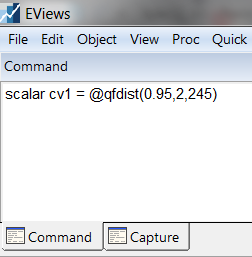
\includegraphics{tute11_44}}
\end{figure}
\vspace{-\baselineskip}
\begin{figure}[H]
	\centerline{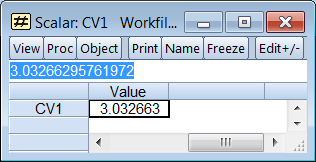
\includegraphics{tute11_45}}
\end{figure}
\vspace{-\baselineskip}
$$F_{crit} =  3.0327$$
\noindent Since $F_{calc} = 4.391 > F_{crit} = 3.0327$ we reject the null at the 5\% significance level and conclude that at least one of the $spread$ lags is significant in explaining $dlgdp$.

\noindent \textcolor{red}{(c) Drop the lag of $spread$ that is least significant \begin{figure}[H]
		\centerline{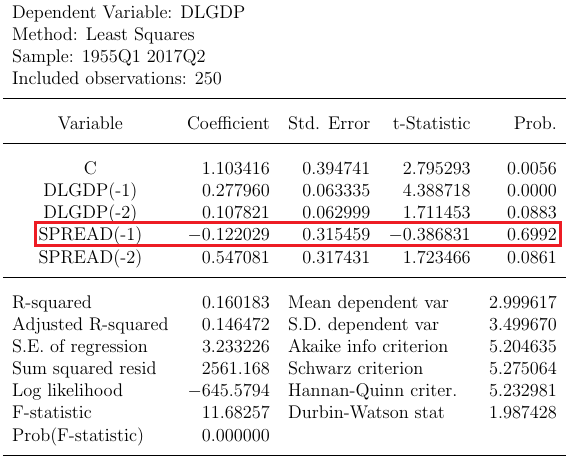
\includegraphics{tute11_46}}
	\end{figure}
	\vspace{-\baselineskip} \noindent and re-estimate the equation. Using this estimated equation, explain the dynamic effect of a 1 percentage point $decrease$ in the spread between long-term and short-term interest rates on the growth rate. In particular, how long does it take for this change to start affecting the growth rate, and what is the long-run effect of this change on the growth rate?}

\noindent The least significant lag of spread is $spread_{t-1}$ so we remove this from the model, $$dlgdp_t = \beta_0 + \beta_1dlgdp_{t-1} + \beta_2dlgdp_{t-2} + \cancel{\beta_3spread_{t-1}} + \beta_4spread_{t-2} + u_t$$ and re-estimate,
$$ls\ dlgdp\ c\ dlgdp(-1to-2)\ spread(-2)$$
%%%%%%%%%% TABLE OBJECT %%%%%%%%%%
\begin{table}[H]
	\centering
	\begin{tabular}{lrrrr}
		\multicolumn{3}{l}{Dependent Variable: DLGDP}&\multicolumn{1}{c}{}&\multicolumn{1}{c}{}\\
		\multicolumn{3}{l}{Method: Least Squares}&\multicolumn{1}{c}{}&\multicolumn{1}{c}{}\\
		\multicolumn{3}{l}{Date: 10/07/18   Time: 17:01}&\multicolumn{1}{c}{}&\multicolumn{1}{c}{}\\
		\multicolumn{3}{l}{Sample: 1955Q1 2017Q2}&\multicolumn{1}{c}{}&\multicolumn{1}{c}{}\\
		\multicolumn{3}{l}{Included observations: 250}&\multicolumn{1}{c}{}&\multicolumn{1}{c}{}\\
		[4.5pt] \hline \\ [-4.5pt]
		\multicolumn{1}{c}{Variable}&\multicolumn{1}{r}{Coefficient}&\multicolumn{1}{r}{Std. Error}&\multicolumn{1}{r}{t-Statistic}&\multicolumn{1}{r}{Prob.}\\
		[4.5pt] \hline \\ [-4.5pt]
		\multicolumn{1}{c}{C}&\multicolumn{1}{r}{$1.058540$}&\multicolumn{1}{r}{$0.376656$}&\multicolumn{1}{r}{$2.810361$}&\multicolumn{1}{r}{$0.0053$}\\
		\multicolumn{1}{c}{DLGDP(-1)}&\multicolumn{1}{r}{$0.281108$}&\multicolumn{1}{r}{$0.062701$}&\multicolumn{1}{r}{$4.483279$}&\multicolumn{1}{r}{$0.0000$}\\
		\multicolumn{1}{c}{DLGDP(-2)}&\multicolumn{1}{r}{$0.111661$}&\multicolumn{1}{r}{$0.062105$}&\multicolumn{1}{r}{$1.797950$}&\multicolumn{1}{r}{$0.0734$}\\
		\multicolumn{1}{c}{SPREAD(-2)}&\multicolumn{1}{r}{$0.438723$}&\multicolumn{1}{r}{$0.149062$}&\multicolumn{1}{r}{$2.943227$}&\multicolumn{1}{r}{$0.0036$}\\
		[4.5pt] \hline \\ [-4.5pt]
		\multicolumn{1}{l}{R-squared}&\multicolumn{1}{r}{$0.159670$}&\multicolumn{2}{l}{Mean dependent var}&\multicolumn{1}{r}{$2.999617$}\\
		\multicolumn{1}{l}{Adjusted R-squared}&\multicolumn{1}{r}{$0.149422$}&\multicolumn{2}{l}{S.D. dependent var}&\multicolumn{1}{r}{$3.499670$}\\
		\multicolumn{1}{l}{S.E. of regression}&\multicolumn{1}{r}{$3.227633$}&\multicolumn{2}{l}{Akaike info criterion}&\multicolumn{1}{r}{$5.197246$}\\
		\multicolumn{1}{l}{Sum squared resid}&\multicolumn{1}{r}{$2562.733$}&\multicolumn{2}{l}{Schwarz criterion}&\multicolumn{1}{r}{$5.253589$}\\
		\multicolumn{1}{l}{Log likelihood}&\multicolumn{1}{r}{$-645.6557$}&\multicolumn{2}{l}{Hannan-Quinn criter.}&\multicolumn{1}{r}{$5.219922$}\\
		\multicolumn{1}{l}{F-statistic}&\multicolumn{1}{r}{$15.58073$}&\multicolumn{2}{l}{Durbin-Watson stat}&\multicolumn{1}{r}{$1.991805$}\\
		\multicolumn{1}{l}{Prob(F-statistic)}&\multicolumn{1}{r}{$0.000000$}&\multicolumn{1}{c}{}&\multicolumn{1}{c}{}&\multicolumn{1}{c}{}\\
	\end{tabular}
	$$\widehat{dlgdp}_t = \underset{(0.3767)}{1.0585} + \underset{(0.0627)}{0.2811}dlgdp_{t-1} + \underset{(0.0621)}{0.1117}dlgdp_{t-2} + \underset{(0.1491)}{0.4387}spread_{t-2}$$
\end{table}
\vspace{-\baselineskip}

\noindent \uline{Using this estimated equation, explain the dynamic effect of a 1 percentage point $decrease$ in the spread between long-term and short-term interest rates on the growth rate. In particular, how long does it take for this change to start affecting the growth rate, and what is the long-run effect of this change on the growth rate?}

\noindent Since $spread_t$ is not included in the model of growth rate, the term spread does not have an immediate effect on the US GDP growth rate. Instead, $spread_{t-2}$ is included, so according to our model, the effect of a change in the term spread on the US GDP growth rate is delayed by 2 periods e.g. it takes 2 quarters before a 1 percentage point decrease in the term spread will affect the US GDP growth rate and when it does, GDP growth is expected to decrease by 0.44 percentage points.

\noindent \textcolor{blue}{In general, the long-run effect on $y$ of a unit increase in $x$ at time $t$ $$= \dfrac{sum\ of\ the\ coefficients\ x_t\ and\ its\ lags}{1 - sum\ of\ the\ coefficients\ of\ lags\ of\ y_t}$$}
\noindent $\therefore$ the $estimated$ long-run effect on $dlgdp$ of a 1 percentage point decrease in the term spread (which is a 1 unit decrease since the term spread is a variable whose unit of measurement is in percentage point) \begin{align*}
	&= \dfrac{sum\ of\ the\ estimated\ coefficients\ of\ x_t\ and\ its\ lags}{1 - sum\ of\ the\ estimated\ coefficients\ of\ lags\ of\ y_t} \\
	&= \dfrac{\hat{\beta}_{spread_{t-2}}}{1-(\hat{\beta}_{dlgdp_{t-1}} + \hat{\beta}_{dlgdp_{t-2}})} \\
	&= \dfrac{0.4387}{1 - (0.2811 + 0.1117)} \\
	&= 0.723\ percentage\ points
\end{align*} 


\noindent \textcolor{red}{(d) Some economists believe that because Central Banks (the Federal Reserve Bank in the case of the US) have become more sophisticated in implementing monetary policy after the mid-1980s, and the informativeness of the $spread$ as a leading indicator has faded. Create an appropriate dummy variable to help you determine that the lag of $spread$ has become insignificant since 1986Q1.}

\noindent To test if $spread_{t-2}$ has become insignificant since 1986Q1, we need to construct the following dummy variable: 
\begin{equation*}
pre86 = \begin{cases}
1 & if\ observation\ is\ before\ 1986 \\
0 & if\ observation\ is\ on\ or\ after\ 1986
\end{cases}
\end{equation*} $$genr\ pre86=@year<1986$$
\begin{figure}[H]
	\centerline{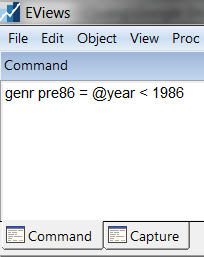
\includegraphics{tute11_47}}
\end{figure} \vspace{-\baselineskip}
\begin{figure}[H]
	\centerline{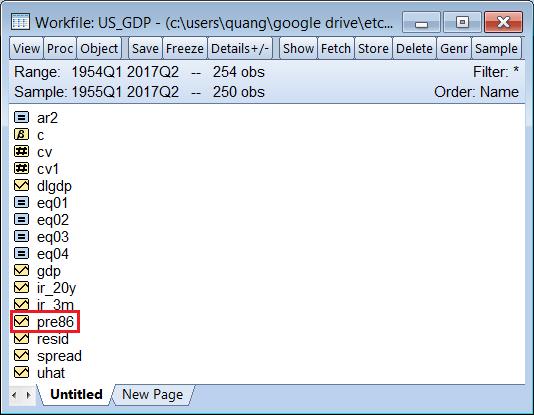
\includegraphics{tute11_48}}
\end{figure} \vspace{-\baselineskip} \noindent and then estimate the following model: $$dlgdp_t = \beta_0 + \beta_1dlgdp_{t-1} + \beta_2dlgdp_{t-2} + \beta_3pre86^*spread_{t-2} + \beta_4(1-pre86)^*spread_{t-2} + u_t$$ with $spread_{t-2}$ once interacted with $pre86$ and once with $(1-pre86)$.

\begin{itemize}
	\item $pre86^*spread_{t-2}$ contains data on the (2nd lag) term spread prior to 1986Q1. i.e. from 1986Q1 onwards, this variable takes on a value of 0, so it only captures information about the term spread pre-1986Q1
	\item $(1-pre86)^*spread_{t-2}$ contains data on the (2nd lag) term spread from 1986Q1 onwards i.e. prior to 1986Q1, this variable takes on a value of 0, so it captures information about the term spread post-1986Q1
\end{itemize}

\noindent If the leading indicator of power $spread$ has deteriorate then we would expect:
\begin{center}
	\textit{The $pre86^*spread$ to be statistically significant in explaining the US GDP growth rate but $(1-pre86)^*spread$ to be statistically insignificant in explain the US GDP growth rate.}
\end{center} 

\noindent $$ls\ dlgdp\ c\ dlgdp(-1to-2)\ pre86^*spread(-2)\ (1-pre86)^*spread(-2)$$
\begin{figure}[H]
	\centerline{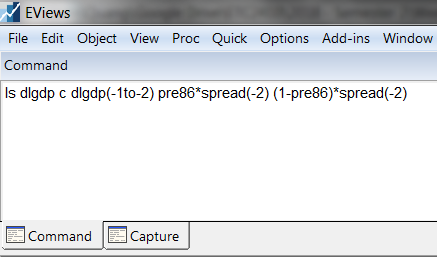
\includegraphics{tute11_49}}
\end{figure} \vspace{-\baselineskip}
%%%%%%%%%% TABLE OBJECT %%%%%%%%%%
\begin{table}[H]
	\centering
	\begin{tabular}{lrrrr}
		\multicolumn{3}{l}{Dependent Variable: DLGDP}&\multicolumn{1}{c}{}&\multicolumn{1}{c}{}\\
		\multicolumn{3}{l}{Method: Least Squares}&\multicolumn{1}{c}{}&\multicolumn{1}{c}{}\\
		\multicolumn{3}{l}{Date: 10/07/18   Time: 18:38}&\multicolumn{1}{c}{}&\multicolumn{1}{c}{}\\
		\multicolumn{3}{l}{Sample: 1955Q1 2017Q2}&\multicolumn{1}{c}{}&\multicolumn{1}{c}{}\\
		\multicolumn{3}{l}{Included observations: 250}&\multicolumn{1}{c}{}&\multicolumn{1}{c}{}\\
		[4.5pt] \hline \\ [-4.5pt]
		\multicolumn{1}{c}{Variable}&\multicolumn{1}{r}{Coefficient}&\multicolumn{1}{r}{Std. Error}&\multicolumn{1}{r}{t-Statistic}&\multicolumn{1}{r}{Prob.}\\
		[4.5pt] \hline \\ [-4.5pt]
		\multicolumn{1}{c}{C}&\multicolumn{1}{r}{$1.211209$}&\multicolumn{1}{r}{$0.362702$}&\multicolumn{1}{r}{$3.339408$}&\multicolumn{1}{r}{$0.0010$}\\
		\multicolumn{1}{c}{DLGDP(-1)}&\multicolumn{1}{r}{$0.203281$}&\multicolumn{1}{r}{$0.062346$}&\multicolumn{1}{r}{$3.260521$}&\multicolumn{1}{r}{$0.0013$}\\
		\multicolumn{1}{c}{DLGDP(-2)}&\multicolumn{1}{r}{$0.078950$}&\multicolumn{1}{r}{$0.059966$}&\multicolumn{1}{r}{$1.316575$}&\multicolumn{1}{r}{$0.1892$}\\
		\multicolumn{1}{c}{PRE86*SPREAD(-2)}&\multicolumn{1}{r}{$1.213964$}&\multicolumn{1}{r}{$0.217398$}&\multicolumn{1}{r}{$5.584054$}&\multicolumn{1}{r}{$0.0000$}\\
		\multicolumn{1}{c}{(1-PRE86)*SPREAD(-2)}&\multicolumn{1}{r}{$0.228862$}&\multicolumn{1}{r}{$0.149687$}&\multicolumn{1}{r}{$1.528941$}&\multicolumn{1}{r}{$0.1276$}\\
		[4.5pt] \hline \\ [-4.5pt]
		\multicolumn{1}{l}{R-squared}&\multicolumn{1}{r}{$0.230086$}&\multicolumn{2}{l}{Mean dependent var}&\multicolumn{1}{r}{$2.999617$}\\
		\multicolumn{1}{l}{Adjusted R-squared}&\multicolumn{1}{r}{$0.217516$}&\multicolumn{2}{l}{S.D. dependent var}&\multicolumn{1}{r}{$3.499670$}\\
		\multicolumn{1}{l}{S.E. of regression}&\multicolumn{1}{r}{$3.095743$}&\multicolumn{2}{l}{Akaike info criterion}&\multicolumn{1}{r}{$5.117730$}\\
		\multicolumn{1}{l}{Sum squared resid}&\multicolumn{1}{r}{$2347.988$}&\multicolumn{2}{l}{Schwarz criterion}&\multicolumn{1}{r}{$5.188159$}\\
		\multicolumn{1}{l}{Log likelihood}&\multicolumn{1}{r}{$-634.7163$}&\multicolumn{2}{l}{Hannan-Quinn criter.}&\multicolumn{1}{r}{$5.146076$}\\
		\multicolumn{1}{l}{F-statistic}&\multicolumn{1}{r}{$18.30431$}&\multicolumn{2}{l}{Durbin-Watson stat}&\multicolumn{1}{r}{$1.999856$}\\
		\multicolumn{1}{l}{Prob(F-statistic)}&\multicolumn{1}{r}{$0.000000$}&\multicolumn{1}{c}{}&\multicolumn{1}{c}{}&\multicolumn{1}{c}{}\\
		[4.5pt] \hline \\ [-4.5pt]
	\end{tabular}
	%\caption{Add your caption here.}
	%\label{tab:}
\end{table}
\vspace{-\baselineskip} \noindent As we can see from the regression output, the term spread has become much less relevant as a leading indicator since monetary policies implementation have been more sophisticated.






\end{document}